% ====================================================================
%
%         Linke Seite Streifen
%
% ====================================================================

    \begin{tikzpicture}[overlay,remember picture]
    \node [
      fill=FFblau,% Farbe des Randstreifens
      text=white,% Textfarbe
      font=\normalfont\bfseries,% Einstellungen für die Schrift
      inner xsep=1em, % Abstand des Textes von unten
      % maximale Textbreite = Papierhöhe - 2*Abstand des Textes von unten:
      text width={\dimexpr\paperheight-2em\relax},
      minimum height=15mm,% Breite des Randstreifens
      anchor=north east,
      rotate=90
      ]
      at (current page.north west)
      {\FFCommunity};           % aus freifunk.sty
  \end{tikzpicture}%

% ====================================================================
%
%         Rechte Seite Streifen
%
% ====================================================================

\begin{tikzpicture}[overlay,remember picture]
    \node [
      fill=FFgelb,% Farbe des Randstreifens
      text=white,% Textfarbe
      font=\normalfont\bfseries,% Einstellungen für die Schrift
      inner xsep=1em, % Abstand des Textes von unten
      % maximale Textbreite = Papierhöhe - 2*Abstand des Textes von unten:
      text width={\dimexpr\paperheight-1em\relax},
      minimum height=25mm,% Breite des Randstreifens
      anchor=north,
      rotate=270
      ]
      at (current page.east){\rotatebox{180}{}};


      % \node[anchor=east, rotate=90] at (current page.east) {};
\end{tikzpicture}

\begin{tikzpicture}[overlay,remember picture]
    \node [
      fill=white,% Farbe des Randstreifens
      text=white,% Textfarbe
      font=\normalfont\bfseries,% Einstellungen für die Schrift
      inner xsep=1em, % Abstand des Textes von unten
      % maximale Textbreite = Papierhöhe - 2*Abstand des Textes von unten:
      text width={\dimexpr\paperheight-1em\relax},
      minimum height=20mm,% Breite des Randstreifens
      anchor=north,
      rotate=270
      ]
      at (current page.east){\rotatebox{180}{}};


      % \node[anchor=east, rotate=90] at (current page.east) {};
\end{tikzpicture}

\begin{tikzpicture}[overlay,remember picture]
    \node [
      fill=FFmagenta,% Farbe des Randstreifens
      text=white,% Textfarbe
      font=\normalfont\bfseries,% Einstellungen für die Schrift
      inner xsep=1em, % Abstand des Textes von unten
      % maximale Textbreite = Papierhöhe - 2*Abstand des Textes von unten:
      text width={\dimexpr\paperheight-1em\relax},
      minimum height=15mm,% Breite des Randstreifens
      anchor=north,
      rotate=270
      ]
      at (current page.east){\rotatebox{180}{Einrichten eines: \routername }};


      % \node[anchor=east, rotate=90] at (current page.east) {};
\end{tikzpicture}


\begin{center}
  \vspace{-1cm}

\includegraphics[scale=1.6]{./site/\FFCommunity/logo.jpg}\\
% Schriftzug Mitte

% \huge{\FFCommunity}\\
%\vspace{0.3cm}

\IfFileExists{./front.pdf}{
\includegraphics[scale=0.25]{./front.pdf}\\}{
\includegraphics[scale=0.25]{./dummy.pdf}\\}
% 
\includegraphics[scale=0.25]{./front.pdf}\\

\routername

\end{center}
\newpage
% \Huge{\FFCommunity} \\

\begin{center}
\IfFileExists{./front.pdf}{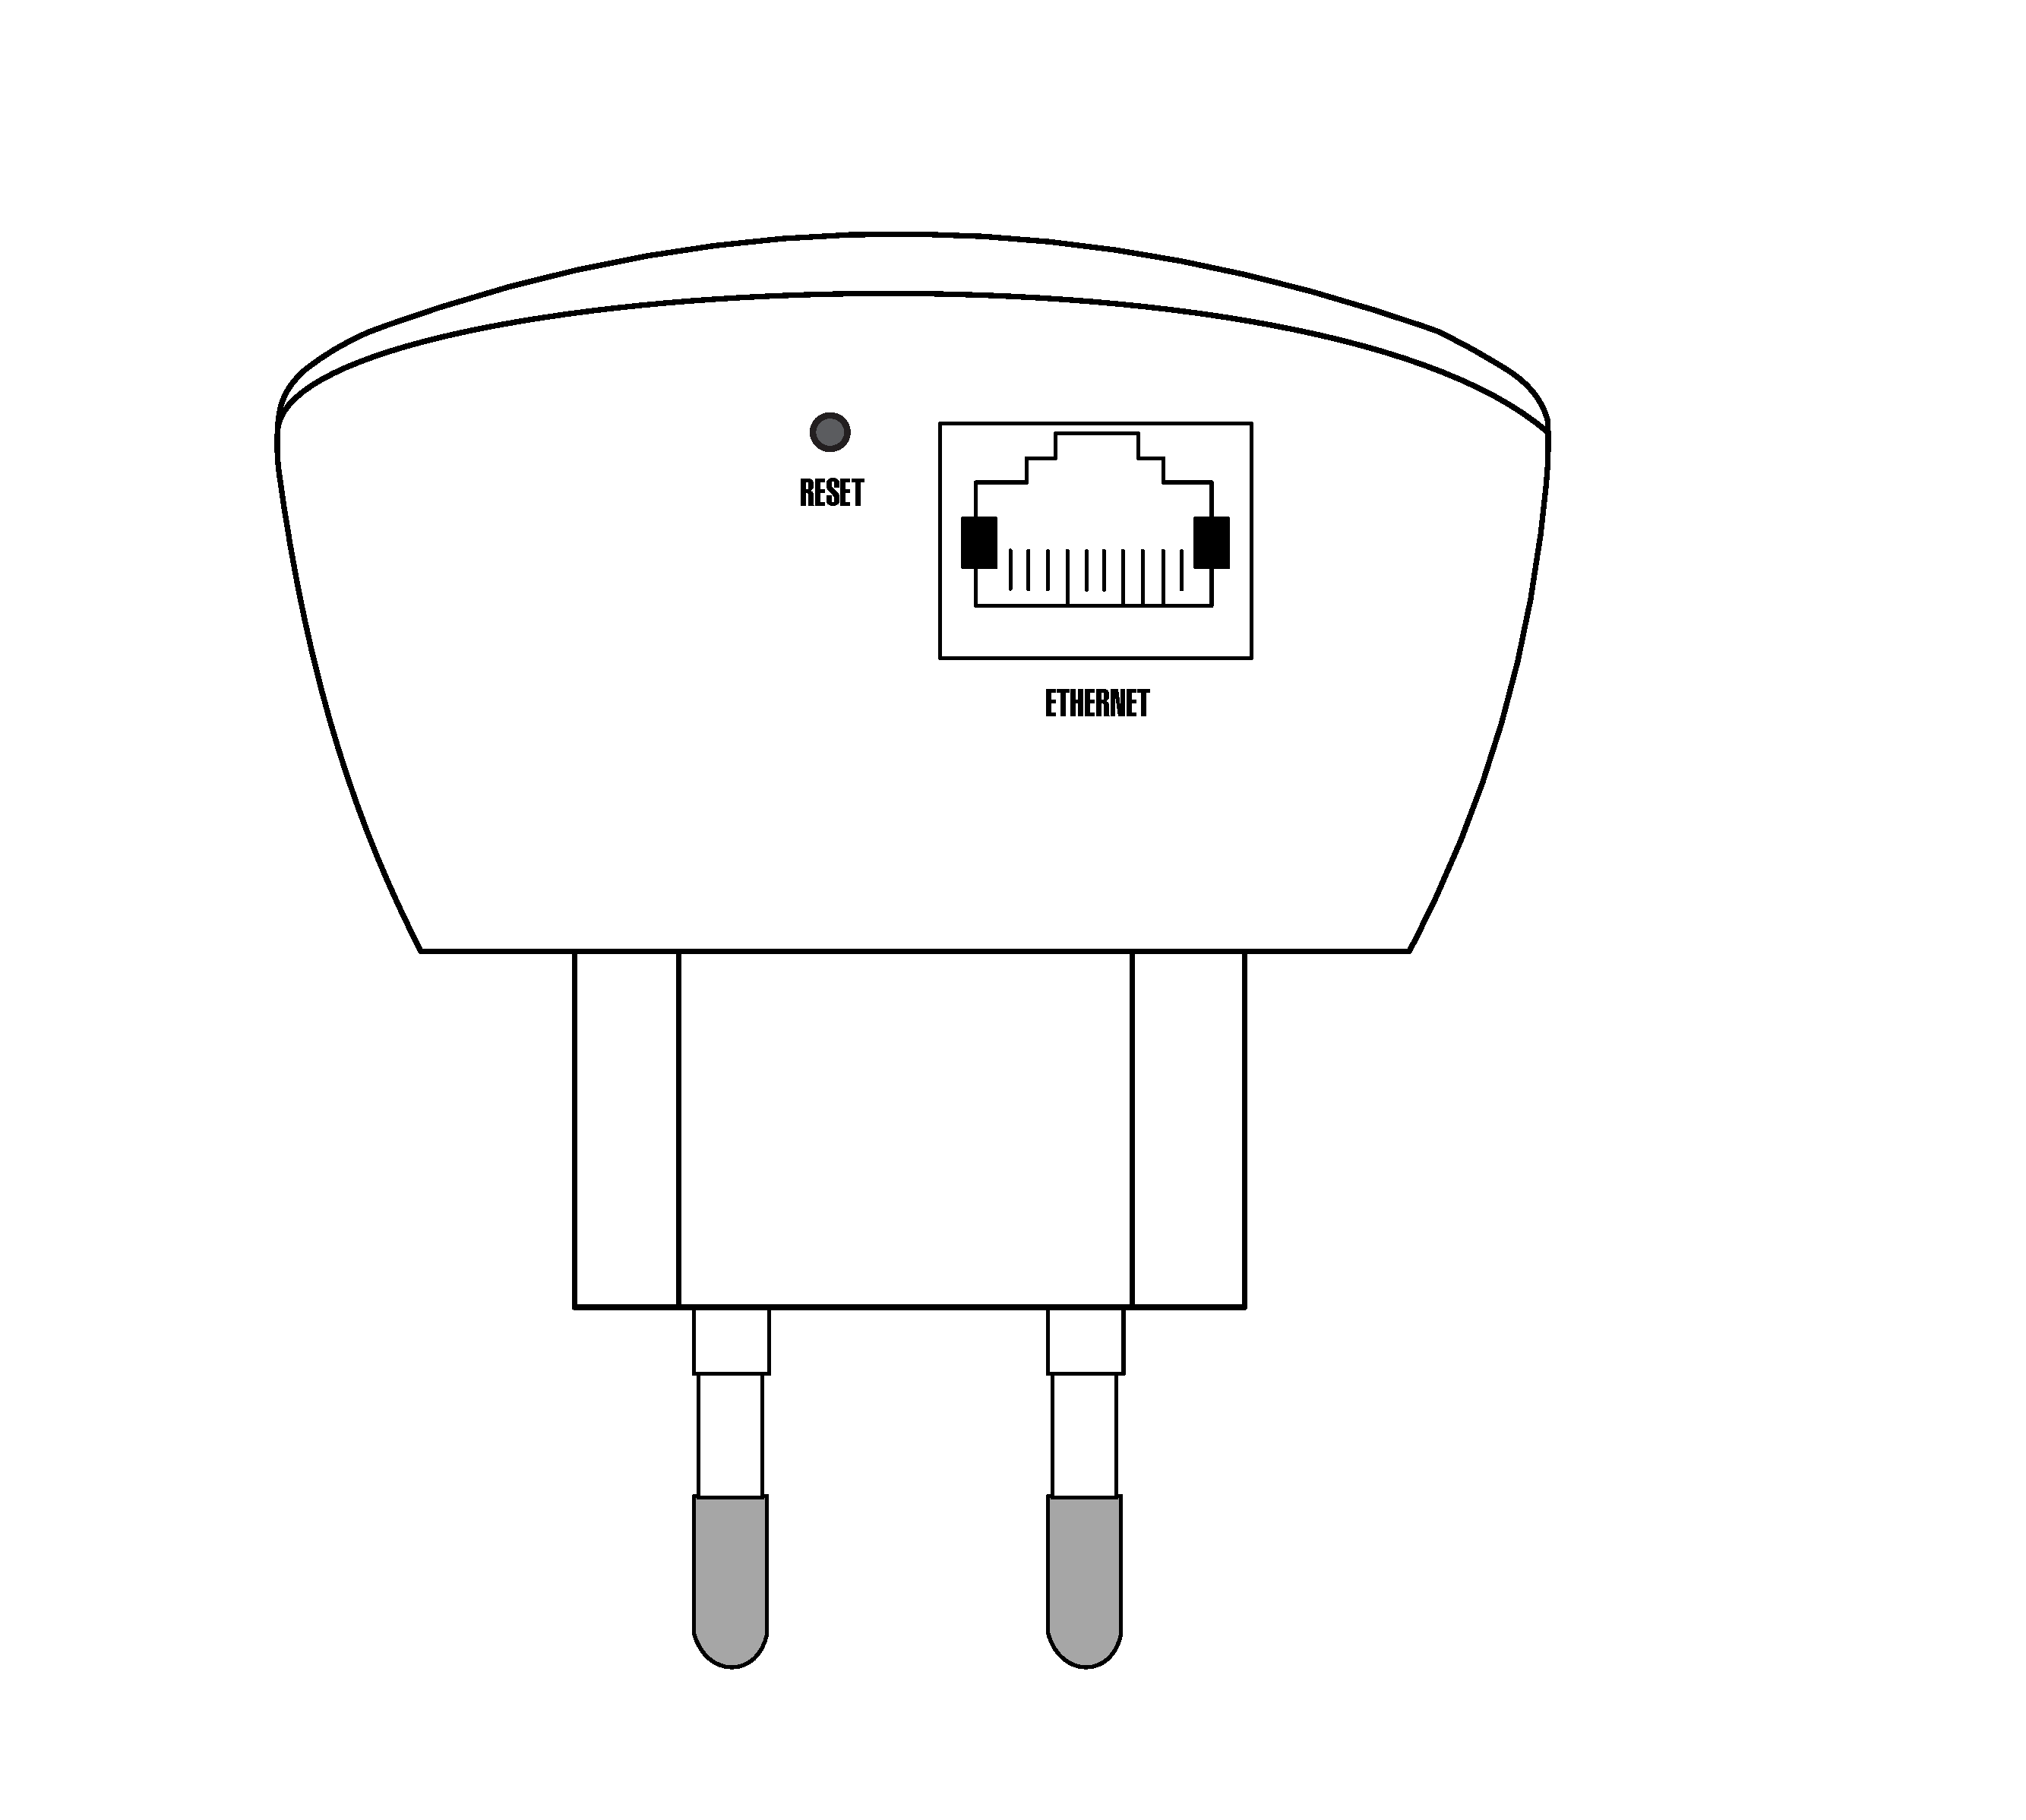
\includegraphics[scale=0.25]{./back.pdf}\\}{
\includegraphics[scale=0.25]{./dummy.pdf}\\}
% 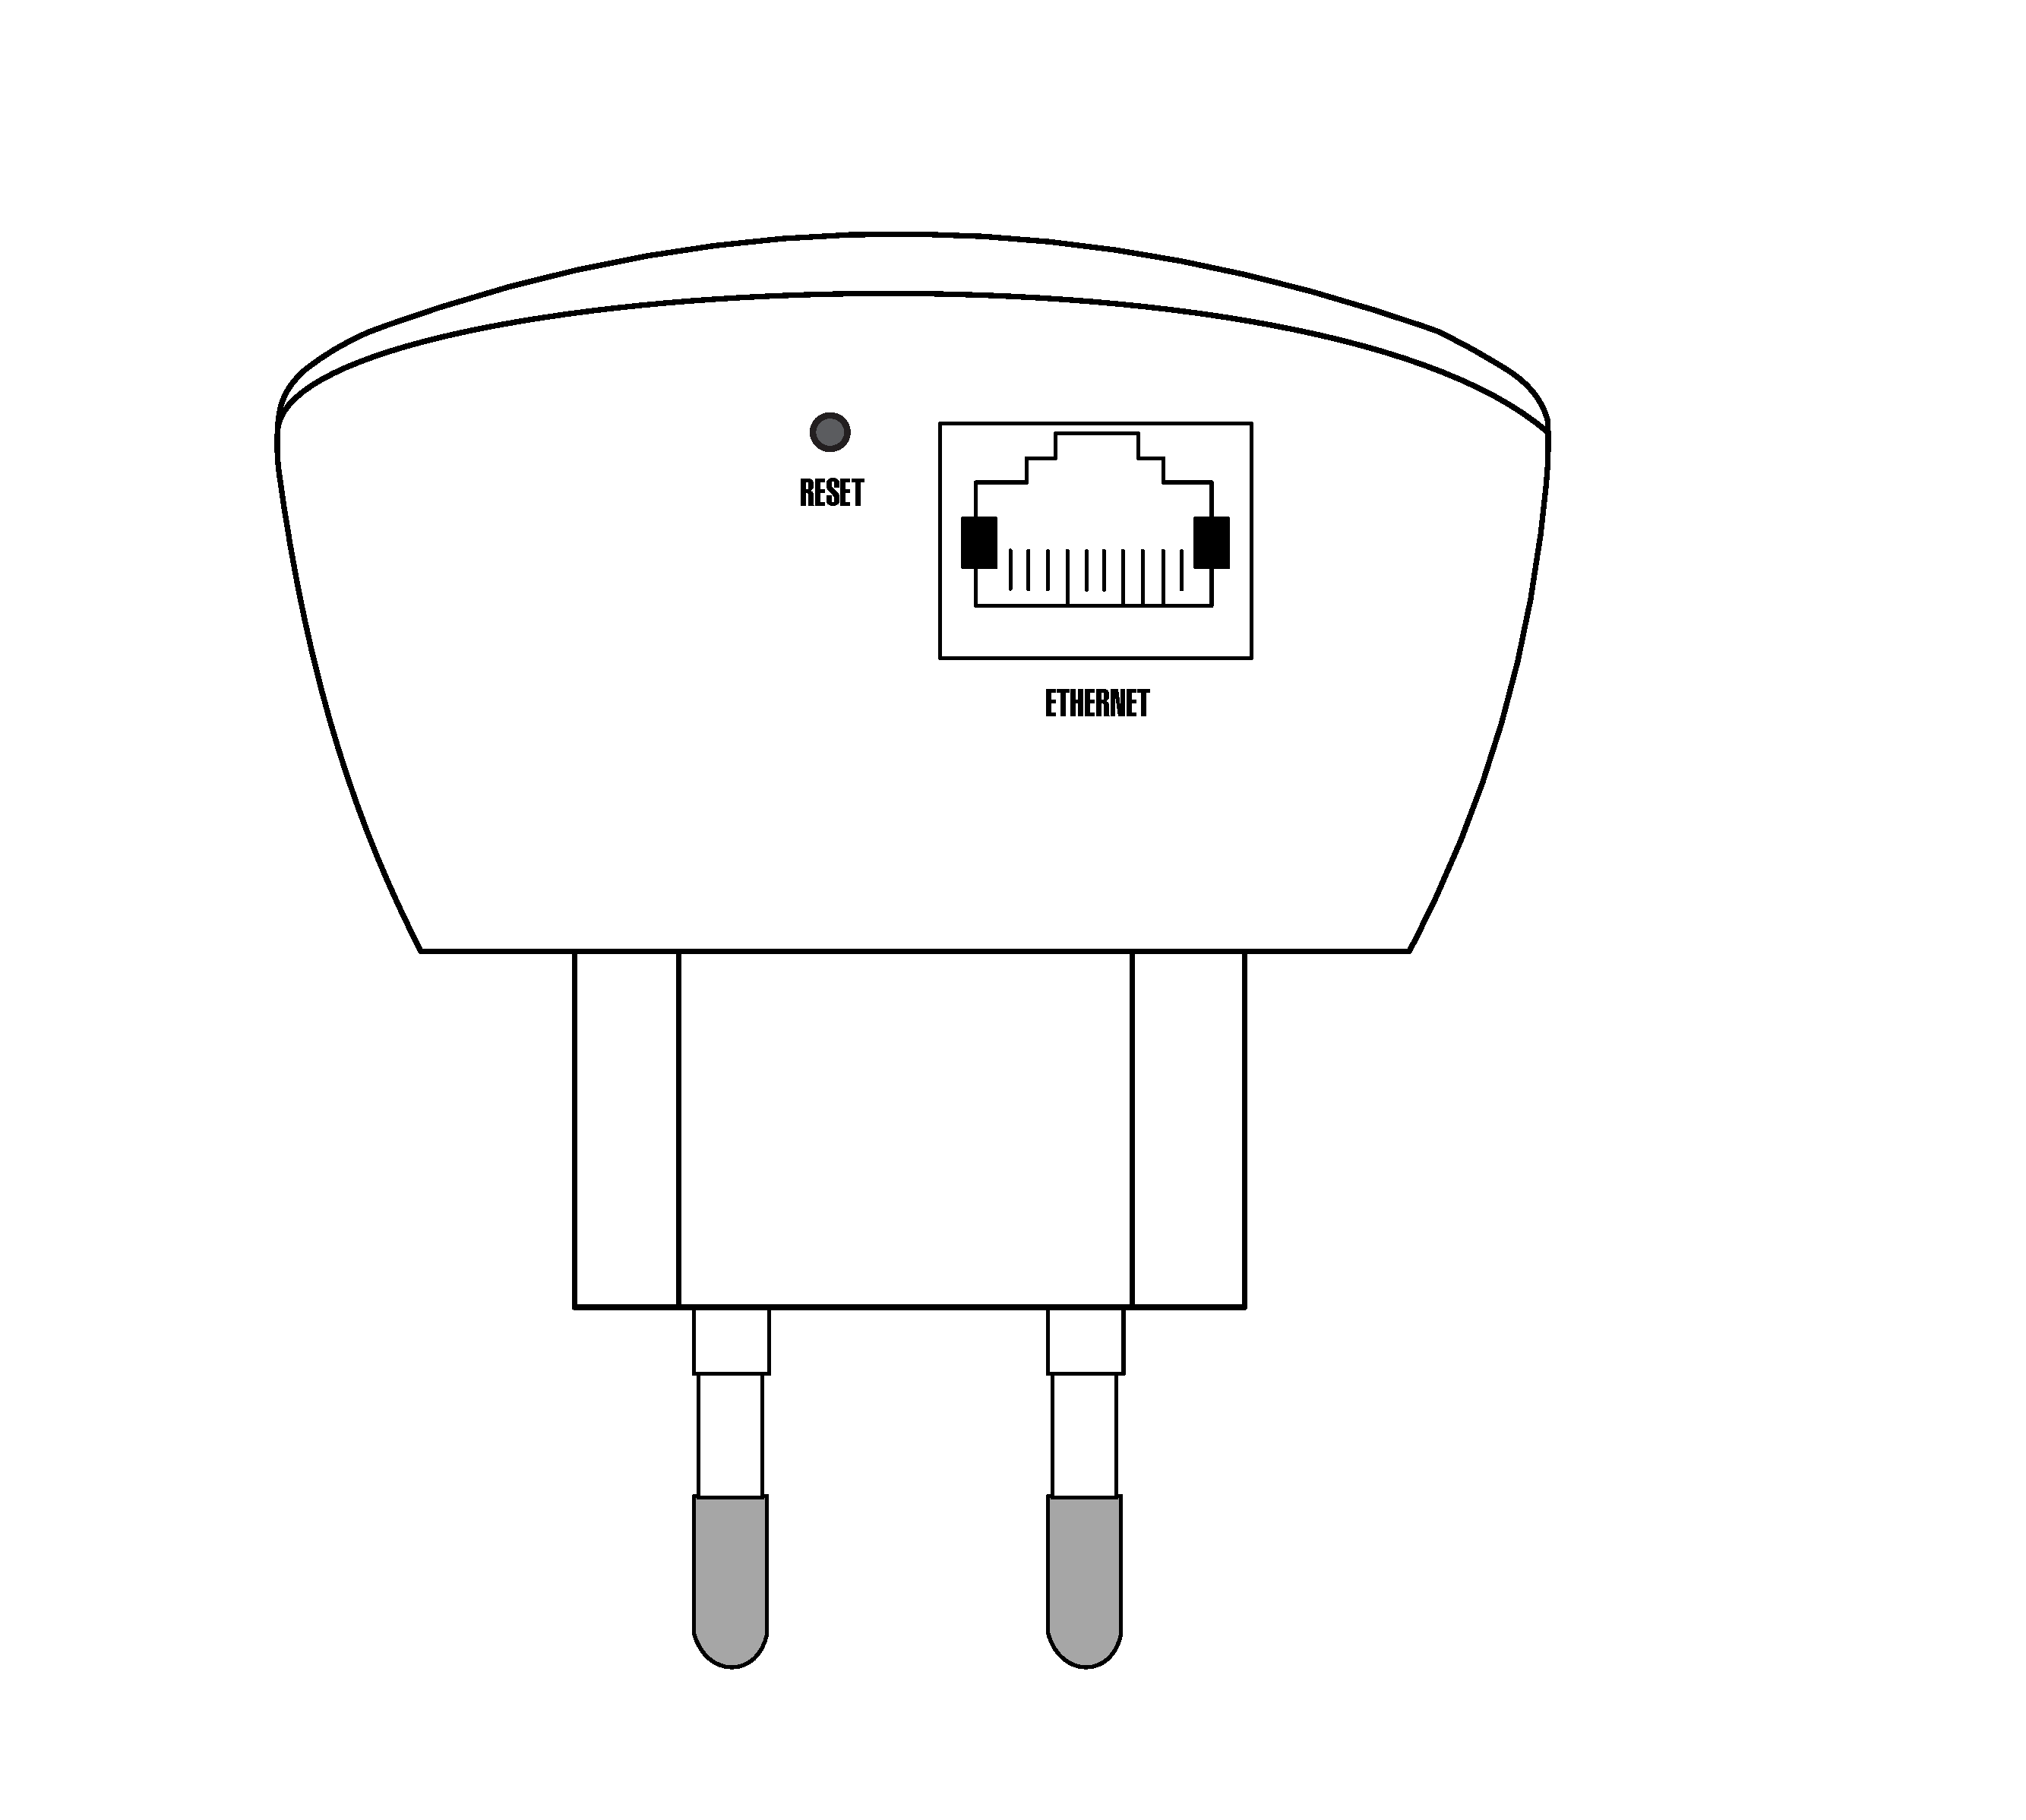
\includegraphics[scale=0.30]{./back.pdf}\\
\Huge{Technische Daten}\\
\end{center}
